\label{sec:hardwareparameters}
\vspace{0.08in}
\noindent{\bf Network topology:}
In this study's experiments, the impact of the hardware design parameters are studied in the context of two 
widely used interconnect topologies: fat-tree and 1D dragonfly.
%Both topologies are used in the current and future HPC systems. 

{\em (1)~1D Dragonfly} -- 1D Dragonfly \cite{Kim2008ISCA}
is a two-level direct network topology: switches form groups with a fully connected
intra-group topology and groups are connected with an inter-group topology.
The topology has three important parameters \cite{Kim2008ISCA}:
the number of compute nodes in each switch ($p$),
the number of links in each switch that connect to other switches in the same group
($a$), the number of links in each switch that connect to other groups ($h$). A balanced dragonfly
in general requires $a = 2p = 2h$. In this study the parameters are set to $p = h = 8$ and $a = 16$.
Each group has 16 switches and 128 compute nodes. 
The global link connectivity between groups follows the per-router arrangement
%with parameters
%(8,1,1) as specified in
\cite{Alzaid2020ICS}.
%For one GPU per node system, the network has
%16 groups and 2048 compute nodes. The number of groups is reduced as more GPUs are
%equipped on each compute node: there are 8 groups
%for 2 GPUs per node case, 4 groups for 4 GPU per node case, and so on. 
The routing algorithm used is the progressive adaptive routing (PAR) \cite{Kim2008ISCA,Alzaid2020ICS}.
% Figure~\ref{fig:dfly_group} show the link connectivity from router R0 in our 1D Dragonfly topology.

{\em (2)~Fat-tree} -- The other topology is a 3-level full bisection bandwidth
fat-tree.  In a 3-level full bisection bandwidth fat-tree, there are three types
of switches: 1)~core switches which are at the top layer to connect pods,
2)~aggregate switches, which connect the leaf switches and form a pod, and
3)~the leaf switches, which are connected to the compute nodes. In a 3-level
full bisection bandwidth fat-tree, the number of uplinks in the aggregate and
leaf switches is the same as the number of downlinks. For our study, the 3-level
fat-tree is built using 32 radix switches. Each leaf switch connects to 16
compute nodes and 16 aggregate switches. Each pod has 16 aggregate switches, 16
edge switches, and 256 compute nodes.
%There are 8 pods in the topology to
%support 2048 compute nodes for 1 GPU per node case, 4 pods for 2 GPU per node
%case, and so on.  We assume adaptive routing for routing of the packets. 

%Figure~\ref{fig:ftree_pod} shows  a fat-tree pod I are use in our
%experiments. We shows the links for L0 and L15 (first and the last leaf
%switch in the pod) and A0 and A15 (first and the last aggregate switch in the
%  pod) to avoid visual clutter. 

\vspace{0.08in}
\noindent{\bf Number of GPUs per node:}
In this study, the number of GPUs in each compute node varies from 1 to
8 to analyze the impact of the increased computation density and the reduction
of network endpoints on the system performance. Each GPU is assigned
to one MPI processes; to simulate different number of GPUs
per node, multiple MPI process are assigned to a node.
The GPUs inside a node are connected in an all-to-all connection topology resembling the intra node connectivity of the Sierra system with NVlink.
The bandwidth between GPUs within a node
is set to be twice the network link bandwidth, so that it replicates that of Sierra supercomputer.
The default setting for GPUs per node is 1 GPU per node. This is the default
GPU per node setting whose performance is used to normalize other results. 
%to which I compare other results.

In the experiments, when I increase the number of GPUs per node, I
proportionally reduce the number of network endpoints, i.e. I make sure that
for all network configurations, the total GPU count, as well the total MPI
  processes, is 2048. This is done
  to ensure that I compare systems that are of computationally equal capability
  as is often the case in the real world. Secondly, I make sure that each
  workload covers the entire network and no node is left empty during the
  simulation. 
  %Note that these configurations were not used for validation
  %purpose, since the validation was done using the exact Quartz supercomputer
  %topology.  
  Table~\ref{table:configs} summarizes the network sizes used for each GPU
  per node setting, with the default setting being that of 1 GPU per node.  

\begin{table}[h]
       \centering
\caption{Network sizes for different GPUs per node.}
        \vspace{-1em}
        \begin{tabular}{ccc} \toprule
        \textbf{GPUs per node} & \textbf{1D Dragonfly} & \textbf{Fat-tree}\\ \midrule 
        1 & 16 Groups & 
        8 Pods \\
        
        2 &
        8 Groups & 
        4 Pods \\
        
        4 & 4 Groups & 
        2 Pods \\
        
        8 & 
        2 Groups & 
        1 Pods\\ \bottomrule
        \end{tabular}
\label{table:configs}
\end{table}


\begin{figure*}[t]
\centering
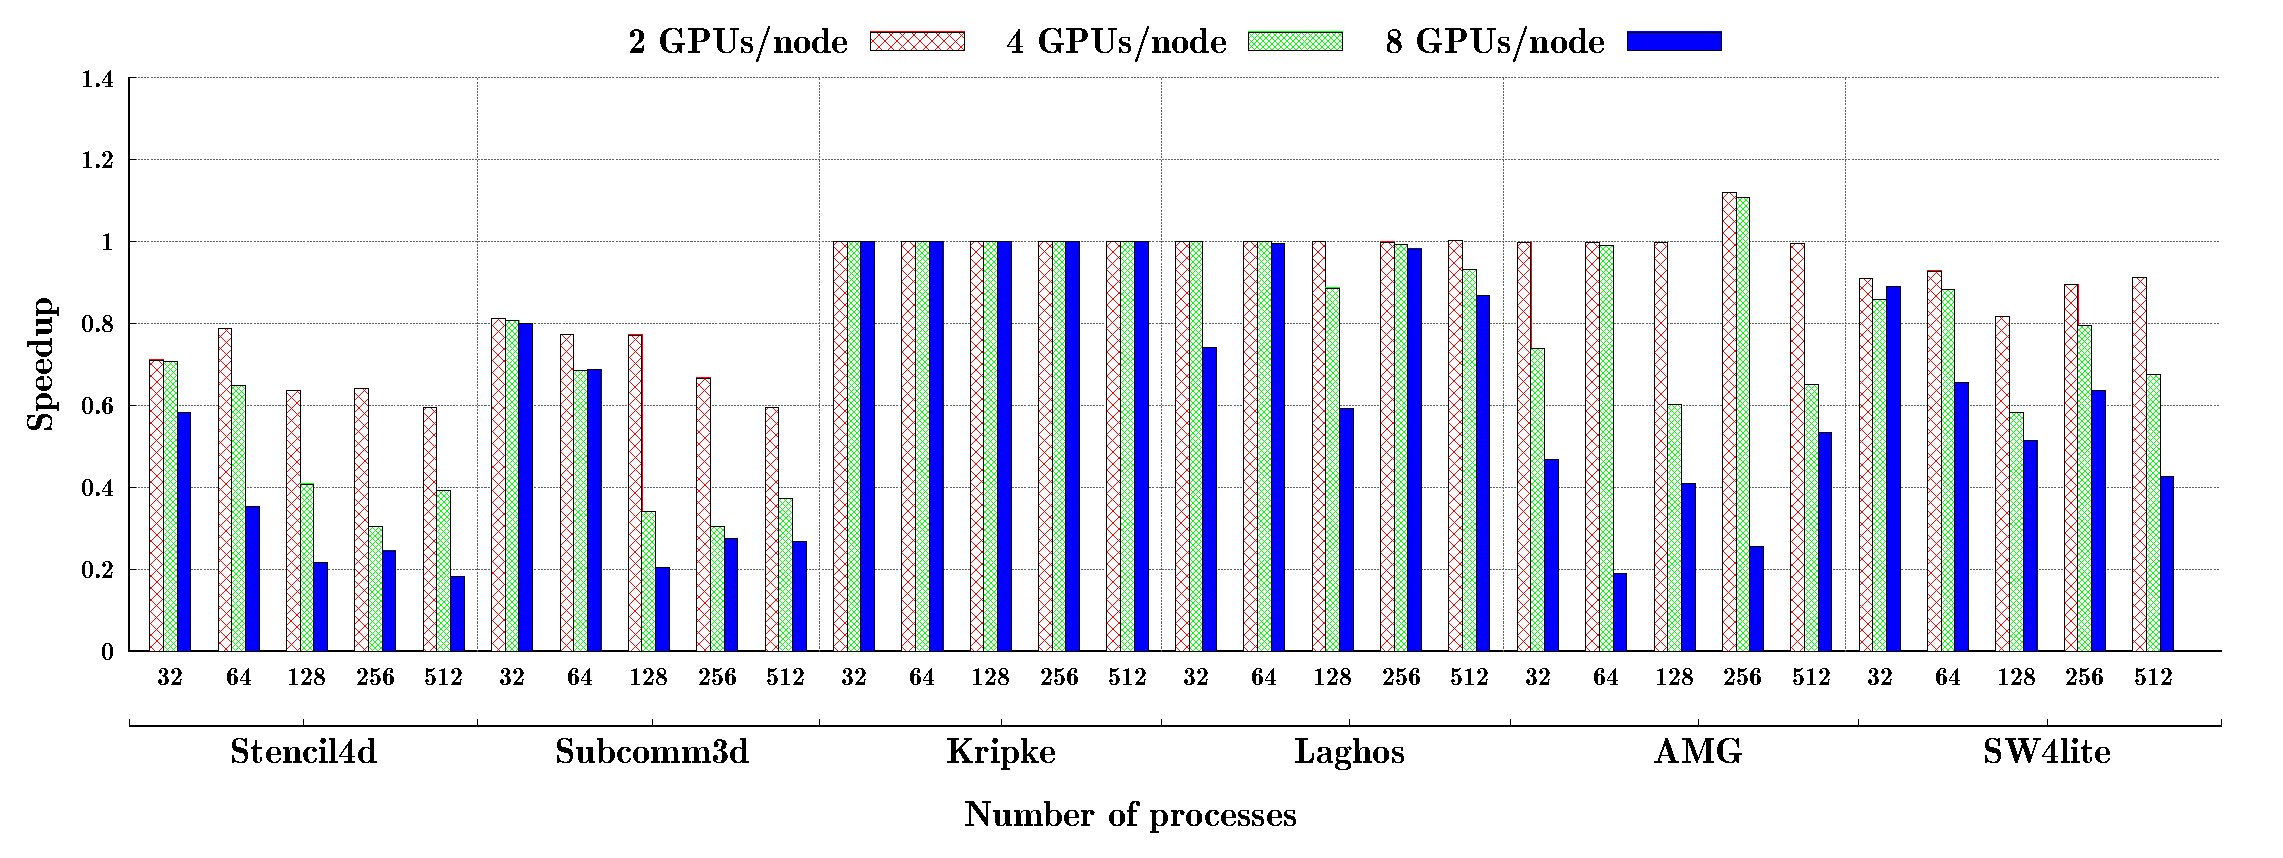
\includegraphics[width=\textwidth]{plots/ftree/map/ftree-mapping-all.eps}
\caption{Speedup on fat-tree for various numbers of GPUs per node settings with
respect to 1 GPU/node configuration.}
\label{fig:ftree_gpu}
\end{figure*}

\vspace{0.08in}
\noindent{\bf Network link bandwidth:}
We set our baseline link bandwidth as x=11.9 GB/s, which is the peak achieved
link bandwidth on Mellanox EDR networks such as
the Quartz supercomputer at LLNL. To analyze the
sensitivity of various compute capability equivalent systems to communication capability, I vary the bandwidth
from x/16 (16 times slow down of the baseline) to 16x (16 times speedup of the
baseline). In the rest of the document, I will use x to represent the base
bandwidth, and will denote the network speed as x/16, x/8, x/4, x/2, x, 2x, 4x,
8x, and 16x.  
%Varying the network speed allows us to quantify the impact of
%increasing network bandwidth for various compute capability equivalent systems.


\vspace{0.08in}
\noindent{\bf Message scheduling:}
As the computation and communication density
on the compute node increases, message scheduling performed by the
NIC may have an impact on
communication performance. In particular, scheduling schemes that alleviate
head-of-line blocking may have significant benefits, especially when the link
bandwidth is very high. In addition to head-of-line blocking, which is often mitigated
by the use of virtual channels, message scheduling also affects congestion management and network
utilization. Scheduling schemes that expose packets from multiple communicating-pairs
to the network may perform better as it provides the network with the flexibility to
use multiple network paths concurrently. To investigate the effect of message scheduling
on a system with different network and different node compute capability, I compare the performance
of FCFS, RR, and RR-N with different values of $N$ on systems with different configurations. 

